\chapter{Model training}
\label{chap:tuning}

In this chapter, we are going to describe our process of developing
the statistical post-editing models. We will take a closer look at the feature selection
methods we have experimented with, the task of model selection and parameter
tuning and also the methods of evaluation we used during the tuning.
We only present experiment results for the separate statistical models,
results of the evaluation of the whole MLFix system is presented in the next chapter.

In this chapter, we will cover following two classification tasks: the identification
of the incorrect instances (words from the MT output with incorrect surface form)
and the prediction of the new morphological categories for the incorrect instances.

Our training process can be separated into three stages: in the first stage, we
focused on choosing a suitable machine learning method, we chose the most promising
one, in the second stage we tried to further increase the performance of the model
based on the chosen ML method by experimenting with various methods of feature filtering
and in the third stage, for each dataset, we search for the best hyperparameters
of the both the selected ML method and feature filtering method.
%We will take a closer look on both stages in the following subsections.


\section{Model evaluation methodology}

We have decided to do word-level evaluation during the model training, more precisely,
we have evaluated the performance of the models using the instances extracted by the
process we described in the previous chapter.

For both error detection and morphological category prediction task, we have defined
a baseline model for comparison. This model basically represents a predictor which
does not detect any errors (all instances are marked as correct) or keeps the original
morphological categories for each instance.

Aside from the standard accuracy metric, we have decided to measure precision and recall
of the trained models. We use standard definition of precision~(\ref{eq:prec-mod}) and recall~(\ref{eq:rec-mod}) using the following equations:
\begin{equation} \label{eq:prec-mod}
precision = \frac{TP}{TP + FP}
\end{equation}
\begin{equation} \label{eq:rec-mod}
recall = \frac{TP}{TP + FN}
\end{equation}
where definitions of \pojem{true positives} (TP), \pojem{false positives} (FP) and \pojem{false negatives} (FN)
vary slightly with each classification task. We also use f-measure to compare combined results of these metrics.

For error detection, each instance which was assigned same value as the \pojem{true prediction}
and different value than the \pojem{baseline} is marked as TP, instance
that was assigned value different both from the \pojem{true prediction} and \pojem{baseline}
is marked as FP and instance with \pojem{predicted value} equal to the \pojem{baseline}
but different from the \pojem{true prediction} is marked as FN.

For the morphological category prediction we use same definition of TP, however, the definitions
of FP and FN are altered in the following way (in both cases, we assume that the \pojem{true prediction}
does not match the \pojem{predicted value}):
\begin{itemize}
\item if the \pojem{baseline} value matches the \pojem{predicted value}, instance is marked as FN,
\item if the \pojem{baseline} value matches the \pojem{true prediction}, instance is marked as FP,
\item if the \pojem{baseline} does not match either one, the instance is marked as i\pojem{wrong positive} WP.
\end{itemize}

The WP is a special case which reflects the situation where predictor tries to predict new value (different
from the original one) but fails and returns just another incorrect value. We must also take into account
the fact, that the error detection classifier is a general model, which is not designed to distinguish
the types of morphological errors and the morphological predictor might be specialized only on a limited
set of the morphological categories. Therefore, sometimes we want it to just leave the \equo{incorrect}
instances unchanged because the reason it was marked as incorrect can be out of its scope.

\section{Automatic error detection}

%data rep - # of features
%cv method
%baseline

We have found that not only during task specification but even during model training,
the task of identifying morphologically incorrect words in the text is more difficult
than the task of assigning the new morphological categories. We have faced several issues
during the training which we will describe in more detail in the following subsections.



\subsection{Unbalanced data problem}

In this task, we face the problem of the binary classification, where we decided
to assign value 0 to the instances that we consider correct and value 1 to the
instances that need to be corrected. The process of assigning these values to the
extracted training instances was described in the previous chapter. 

%For the model evaluation, we defined a baseline classifier, which assigned the 0 value
%to each instance, therefore marking all of the MT output as already correct.
In this task, the \pojem{baseline classifier} already achieved accuracy larger than 95\%
simply by marking all the instances as correct.
As we have already pointed out, this is because only a small portion of our
training instances is marked as incorrect by our heuristic.
This became a severe issue since most of the machine learning methods rely more or less on accuracy during
the process of searching for the best hypothesis, however, it is the minority
class, that is our target during the error classification.

There are several methods that can be used to solve this problem\todo{citace?}: e.g. creating syntetic
training data by resampling instances with our minority class or removing some instances
belonging to the dominating class, weighting of the training instances or modification of the
cost function. The manipulation with the training data (upsampling, downsampling) is the easieast method,
however, the more it modifies the distribution of the classes over the training data, the worse can become the final
performance of the classifier on the real-life data. Still, the idea of modifying the distribution
of our training data is worth considering.

We have inspired ourselves in the work of Jia describing the classification of grammar errors in the texts
written by a human\cite{biblio:ZaPoHiddenMarkov2009}. They are aproaching the task, similarly to us, as an classification
problem. During training, they filter their training corpus using only around 5\% of
the sentences, because only those were the ones that contained grammatical errors.

In our case, if we look at the results produced by the Oracle classifier, we can see that at least
two-thirds of the MT sentences have not been modified. This means that at least two-thirds of the sentences
were considered morphologically \equo{correct}\footnote{This is very likely not to be true, but can at least assume
that they do not contain training instances marked as incorrect (as far as our heuristic goes).}
These sentences are still part of our original training data introducing a significant amount of training
instances marked as correct.
Therefore, to balance our data, we have decided to use only the training
instances from the sentences where at least one word was marked as incorrect. This way, we were
able to increase the portion of the minority class up to 10\%.

This less unbalanced dataset, we have created this way can be used in two ways: we can simply treat
it like a downsampled data and use the trained models \equo{globally} (on every MT sentence),
or we can rather add another component that will be used to identify these \equo{incorrect} sentences
and than apply our error detection model.

%This obviously creates another task and that is detection of the \equo{incorrect} sentences.

%%% TOTO UZ JE ZMINENE NA ZACATKU %%%
%Our training process can be separated into two stages: in the first stage, we
%focused on choosing a suitable machine learning method, we chose the most promising
%one and in the second stage we tried to further increasing the performance of model
%based on the chosen method by experimenting with various methods of feature filtering.
%We will take a closer look on both stages in the following subsections.

\subsection{Machine learning method comparison}

There are many machine learning methods that support binary classification, so we
decided to only compare a limited subset of the available methods that are implemented
in the Scikit-Learn framework. For each classifier we tried several hyperparameter
settings to observe the changes in the classifier behaviour. However, we have made only
a rough examination of the hyperparameter configuration due to the number of observed
methods. In this stage, the goal was not to train the best possible classifier but
eliminate those, that are not suitable for the task.

We have tried to measure the performance of the classifiers on several datasets. We have used
the WMT10 data, dataset extracted from the lingea logfiles (HimL) and
WMT16 newstest dataset translated by the Chimera system.
For each datasets, only instances from the \equo{incorrect} (sentences contaning at least one error)
sentences were used.
%one translated with the experimental neural network machine translation system (NMT)
%provided by the University of Edinburgh\todo{no ref, nezminovat?}.
Additionally, a counterpart was
created by substitution of the reference sentences with the Depfix output
to additionally measure the performance on the \equo{syntetic} data.
The summary of the size of the used training data is in~\Tref{wf-training-sum}

\begin{table*}[t]
\centering
\small

\begin{tabular}{lcc}
Dataset  &  \hash{} Instances  &  \hash{} Instances (filt.)  \\
\hline
WMT10  &  23,470  &  6,033  \\
HimL  & 7,234  &  2,469  \\
WMT16-chimera  &  26,942  &  7,047  \\
WMT10-Depfix  &  40,678  &  4,101  \\
HimL-Depfix  &  10,491  &  1,114  \\
WMT16-chimera-Depfix  42,021  &  1,897  \\
\end{tabular}
\caption{
    Summary of the size of the training data extracted from each dataset. We present
size before and after (filt.) removing the instances extracted from the \equo{correct} sentences.
}
\label{wf-training-sum}
\end{table*}


For the purposes of the coarse evaluation we used each dataset separately for both training
and testing of the classifers, by performing one-against-the-rest 10-fold jackknife sampling.
Therefore the results presented in this stage should be considered only as an in-domain
performance for a specific MT system.

We have compared the following methods\todo{reference k metodam?}: logistic regression, ridge regression classifier,
random forests, extremely randomized trees and support vector machines (SVM) classifier.
In the~\Fref{wf-draft}, we can see the comparison of the performance of various classifiers based
on the F1-measure metric. We can see, that for the task of error identification, the support vector
machines with linear kernel might be the most suitable overperforming other methods in most of our
datasets. The \equo{baseline} peformance is not spectacullar, with score of less 0.3 for the normal data
and a slightly better score (\tilda{}0.5) for the Depfix data. Therefore we have decided to explore
further only SVM during the following stages of model training.

% with source
\begin{figure}
\centering
  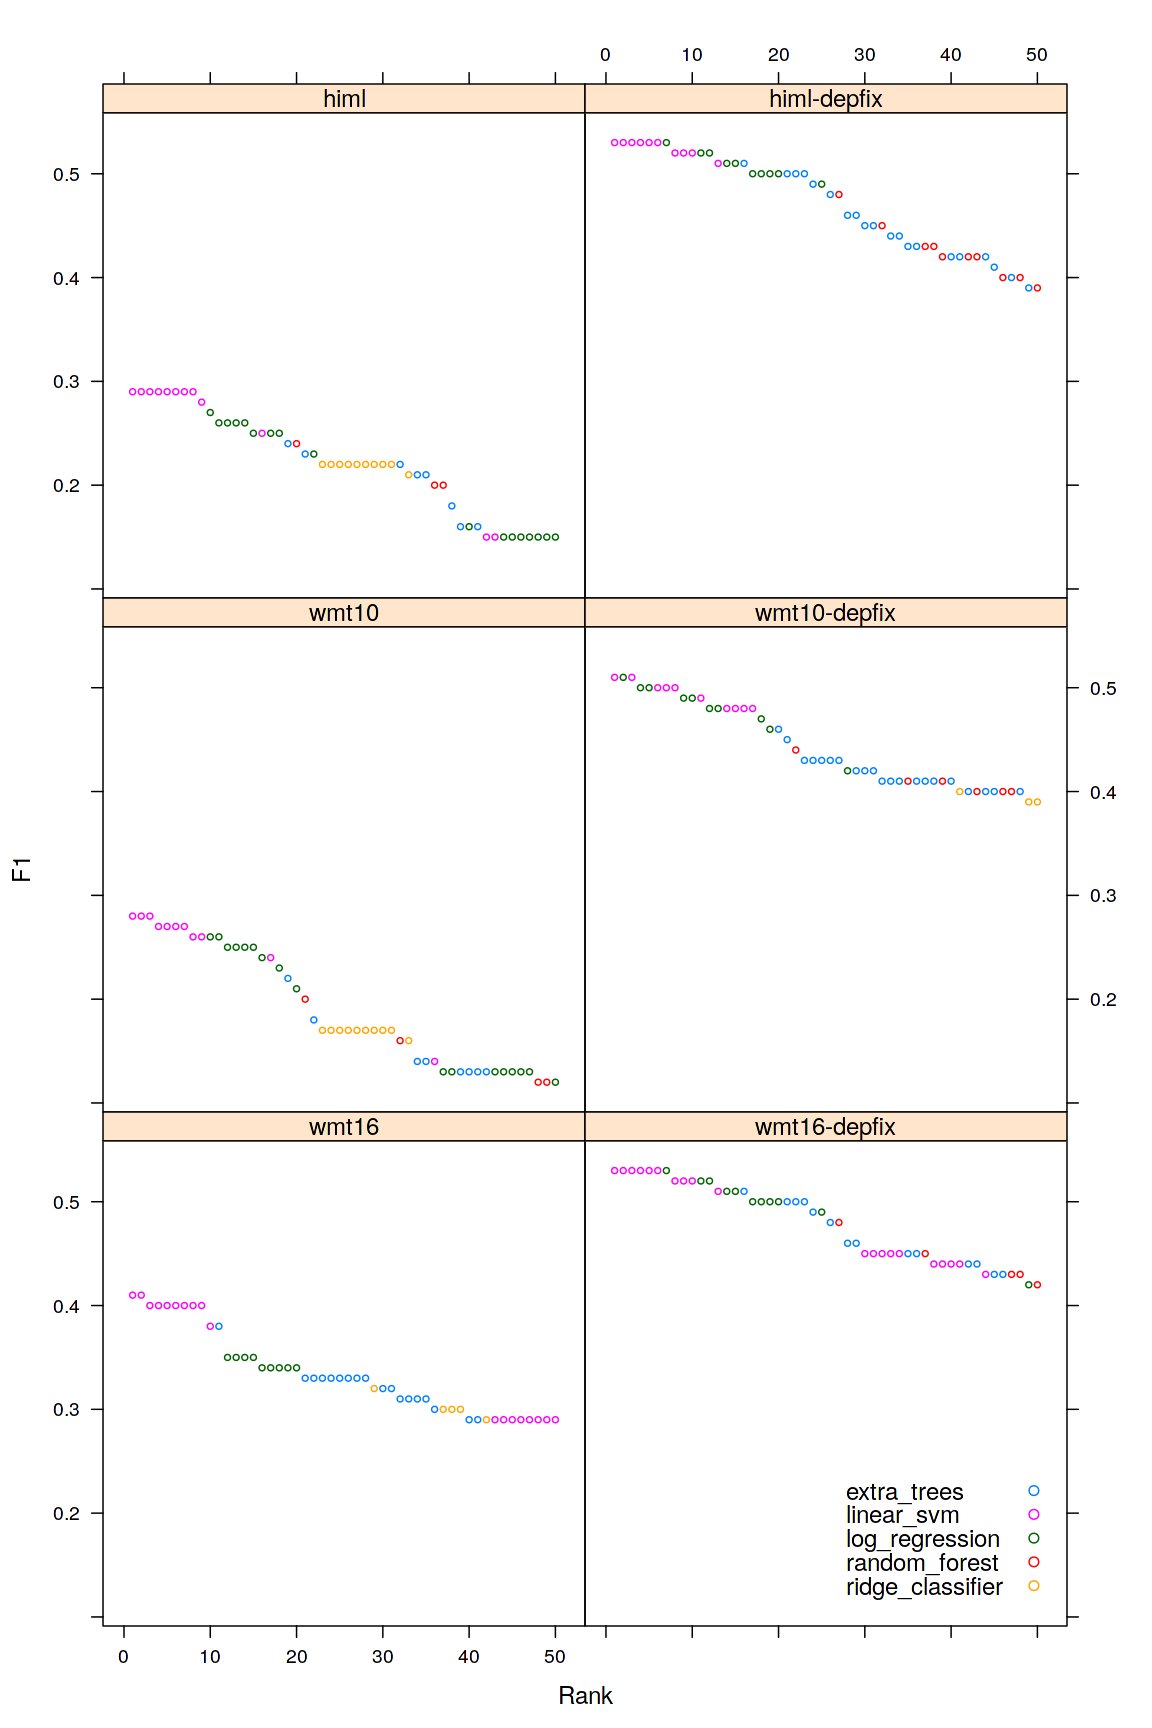
\includegraphics[scale=0.7]{wf-class}
  \caption{
    Overview of the classifier performance (error detection).
We have tried several variations of the hyperparameters
for each classifier. The classifiers are ordered from the best to the worst. Only top 50 results
are shown for each dataset.
}
  \label{wf-draft}
\end{figure}

\subsection{Feature filtering}

During the model comparison, we have compared performance on two initial feature sets:
one did not contain any information about the source sentence (\tilda{}680 initial features)
and one with the source sentence features (\tilda{}1360 initial features). Before training
the features with zero variance were removed, however, no other feature selection has been
performed. We have noticed that the additional information provided by the source sentence features
significatnly improves performance of the majority of the ML methods. Therefore, we have decided
to use this feature set for the feature selection method comparison.

We have picked SVM as ML of our choice. We have picked several methods for feature
selection and compared their influence on the classifier performance. During the comparison
we used a SVM model with fixed hyperparameters. We compared the following methods for
feature selection: KBest selection (with chi-squared scoring function), selection of the percentile
of the features (based on the ANOVA F-test),
selection based on lasso regularization and selection through models with feature importance
scoring models (svm, random forest). As far as importance scoring goes, we compared different
model configurations and during features selection, only features with importance higher
than the mean of the feature importance distribution were selected.

The results of the feature selection method comparison are shown in~\Fref{wf-sel}. We can see
that most of the time the feature selection performed by either ANOVA percentile selector or
SVM slightly improved the model performance. We have therefore decided to investigate this methods
further.

\begin{figure}
\centering
  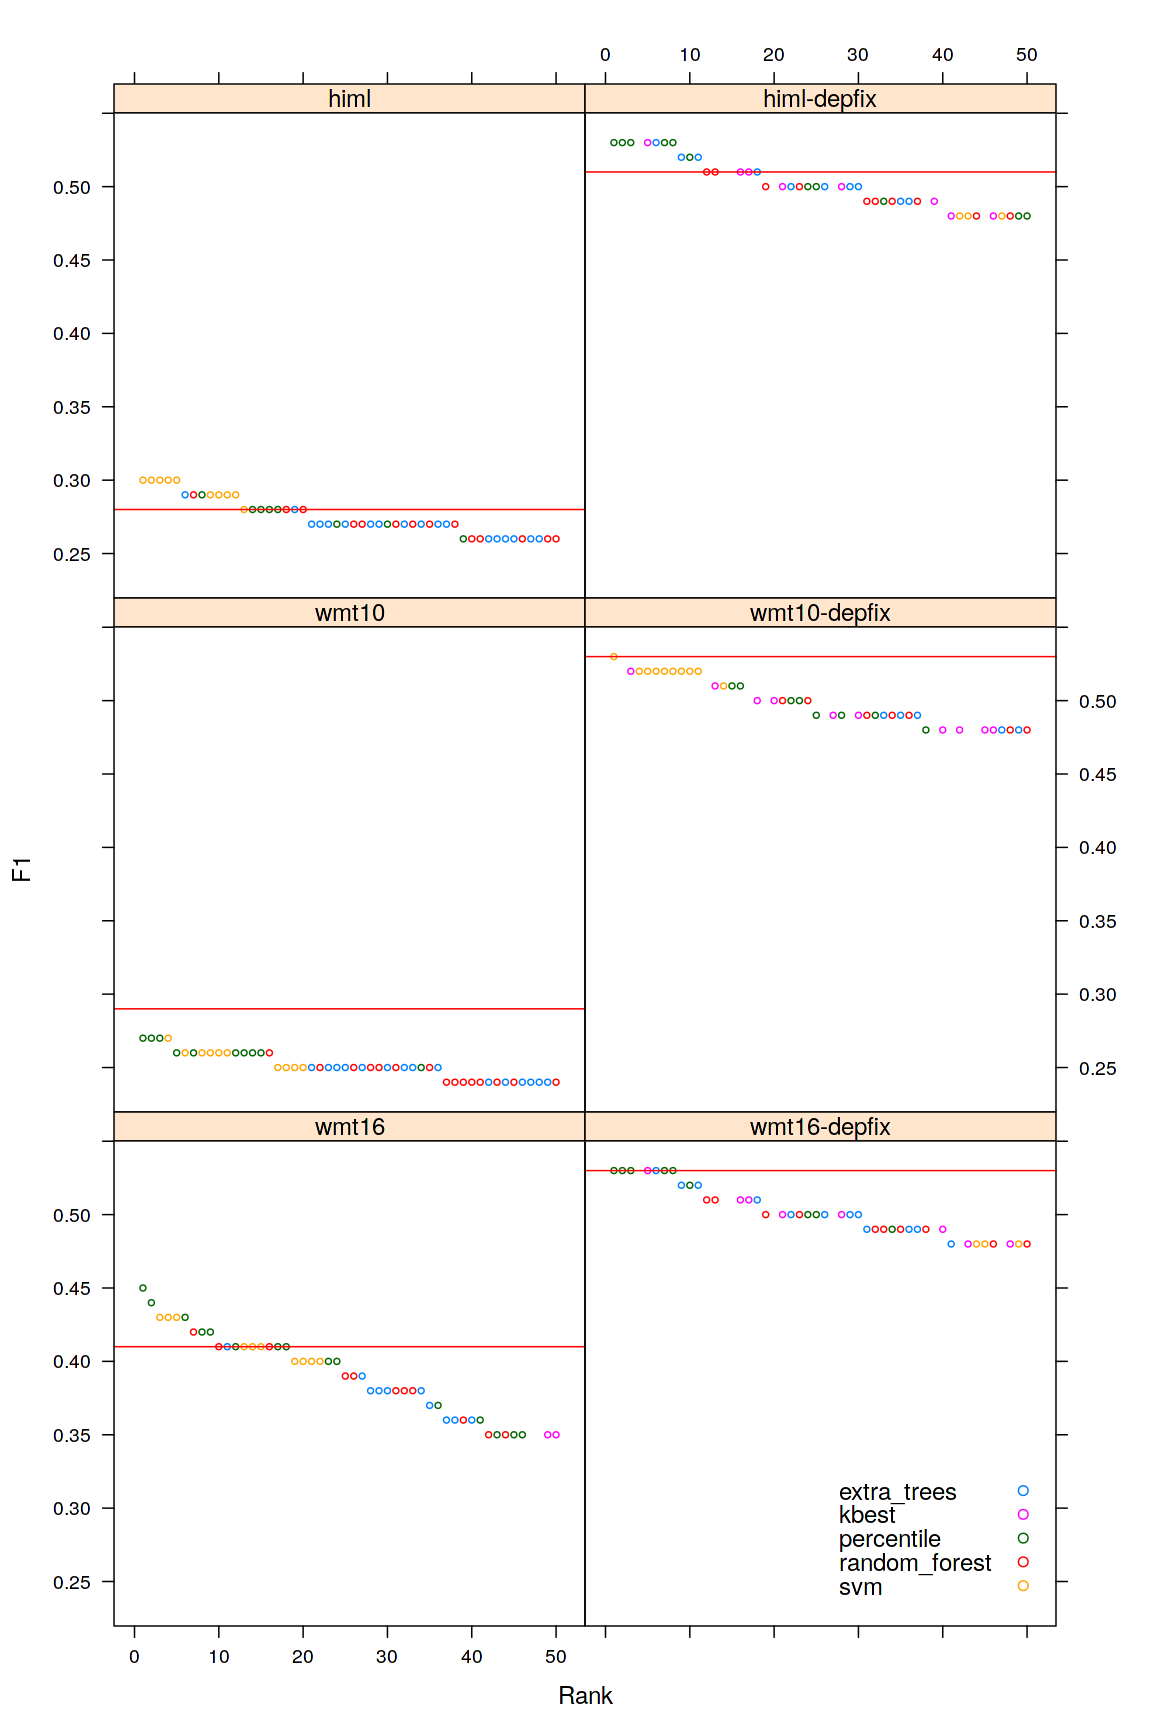
\includegraphics[scale=0.7]{wf-sel}
  \caption{
    Overview of the performance of the SVM with linear kernel when combined with various feature selection methods.
We have tried several variations of the hyperparameters
for each method. The horizontal line marks the best performance without
a feature selection method. The methods are ordered from the best to the worst. Only top 50 results
are shown for each dataset.
}
  \label{wf-sel}
\end{figure}

%TODO: feature representation - vectorized dicts, binary features???
% chceme to zminovat?

\subsection{Model summary}



\section{Prediction of new categories}

The second classification problem was predicting the correct morphological category for
the words that were marked as incorrect. Because we are using the Interset representation
of the morphological features we have several possibilities, how to handle this task such
as:
\begin{enumerate}
    \item predict each category separately,
    \item concatenate the features and treat them as a single prediction target,
    \item use the methods that support multitask classification,
\end{enumerate}

With the first option, the biggest issue is determining the order in which the classifiers
should be aplied. Additionally we have to decide if we also want to include the current node morphological features
into our model's feature set or use the newly predicted ones. The second approach eliminates this problem by predicting the
values simultaneously. This can, however, quite easily expand the set of the predicted values,
which usually leads to increase in data sparsity. This can be a big problem as we have
already shown that the amount of data available for the post-editing task (mainly the post-edited
data) can be quite low. The third option combines the first two by training an estimator
which handles multiple joint classification tasks, one for each morphological category. The
Scikit-Learn toolkit provides several classifiers which support this option.

Before jumping straight into training our classifier, it is important to examine what morphological
changes are made in our training data, how frequent they are and how can they affect the resulting
surface form generation. We can, for instance, predict new values of the \samp{punctype} category,
but it is almost certain that it will not affect the resulting wordform of any of the words
classified as incorrect, because this category is related strictly to punctuation. There are
of course less obvious examples and some categories, while being relevant for one target language
can be pointless in another.

For this reason we made a frequency analysis of the changes encountered
in our data, shown in the~\Fref{iset-barplot}. We can see that most of the time, only the grammatical
case was modified (more than 50\% of the instances for the Depfix-based datasets and more than 40\% of the instances for
the normal datasets). Other changes were a lot less frequent (less than 10\% of the modified instances).
We have also checked, how often was each POS being changed. \Tref{changes-pos} summarizes the change frequencies for each
POS. As a conclusion we have decided to focus on predicting these categories: grammatical case, number, gender
and animateness.

\begin{table*}[t]
\centering
\small

\begin{tabular}{lc}
POS  &  Frequency  \\
\hline
noun    &   38\%  \\
adj     &   16\%  \\
adp     &   10\%  \\
verb    &   9\%  \\
adv     &   9\%  \\
\end{tabular}
\caption{
    Part-of-speech (POS) frequencies of the changed words.
}
\label{changes-pos}
\end{table*}


\subsection{Machine Learning method comparison}

We have decided to train four models: one predicting case only (C), one predicting case and number (CN),
 one predicting case, number and gender (CNG) and one predicting case, number, gender and animateness (CNGA).
We have used same datasets as in the previous task, however, this
time we have extracted only feature vectors of the instances that were marked as incorrect in our training data. Because
our predictors will only be classifying the incorrect instances, training them on the whole dataset would only create
unnecesary bias. On the other hand, this has made the training sets quite small (containing only a few hundreds of examples
at most). The summary of the training data is in~\Tref{cats-training-sum}. We have decided to train a separate classifier
for each dataset instead of combining the data together, because we can simply combine the models instead (e.g. via majority
vote, best prediction etc.). This allows us evaluating the combined model of a test set of our choice simply by leaving
out the model which was trained on that specific test set.

\begin{table*}[t]
\centering
\small

\begin{tabular}{lc}
Dataset  &  \hash{} training instances  \\
\hline
WMT10  &  645  \\
HimL  & 338  \\
WMT16-chimera  &  722  \\
WMT10-Depfix  &  210  \\
HimL-Depfix  &  72  \\
WMT16-chimera-Depfix  &  99  \\
\end{tabular}
\caption{
    Summary of the size of the training data extracted from each dataset.
}
\label{cats-training-sum}
\end{table*}

Again, we had to decide which ML method should we use for this task. 
We have examined similar set of classifiers with similar
hyperparameters as in the error classification task to get a rough idea about their capabilities. We compared them mainly
through their f-measure performance.
The rough comparisons were made with the case classifier only,
we have assumed, that the ML performace will be similar for the other two categories.
The results are shown in~\Fref{cats-draft}. We can see, that even without any sophisticated parameter
tuning or feature filtering, the classifiers perform quite well. We can also notice that in most of the cases, the ensemble
methods (random forests, extremely randomized trees) performed slightly better than the rest. Therefore we have decided
to pick these methods for further experiments.

\begin{figure}
\centering
  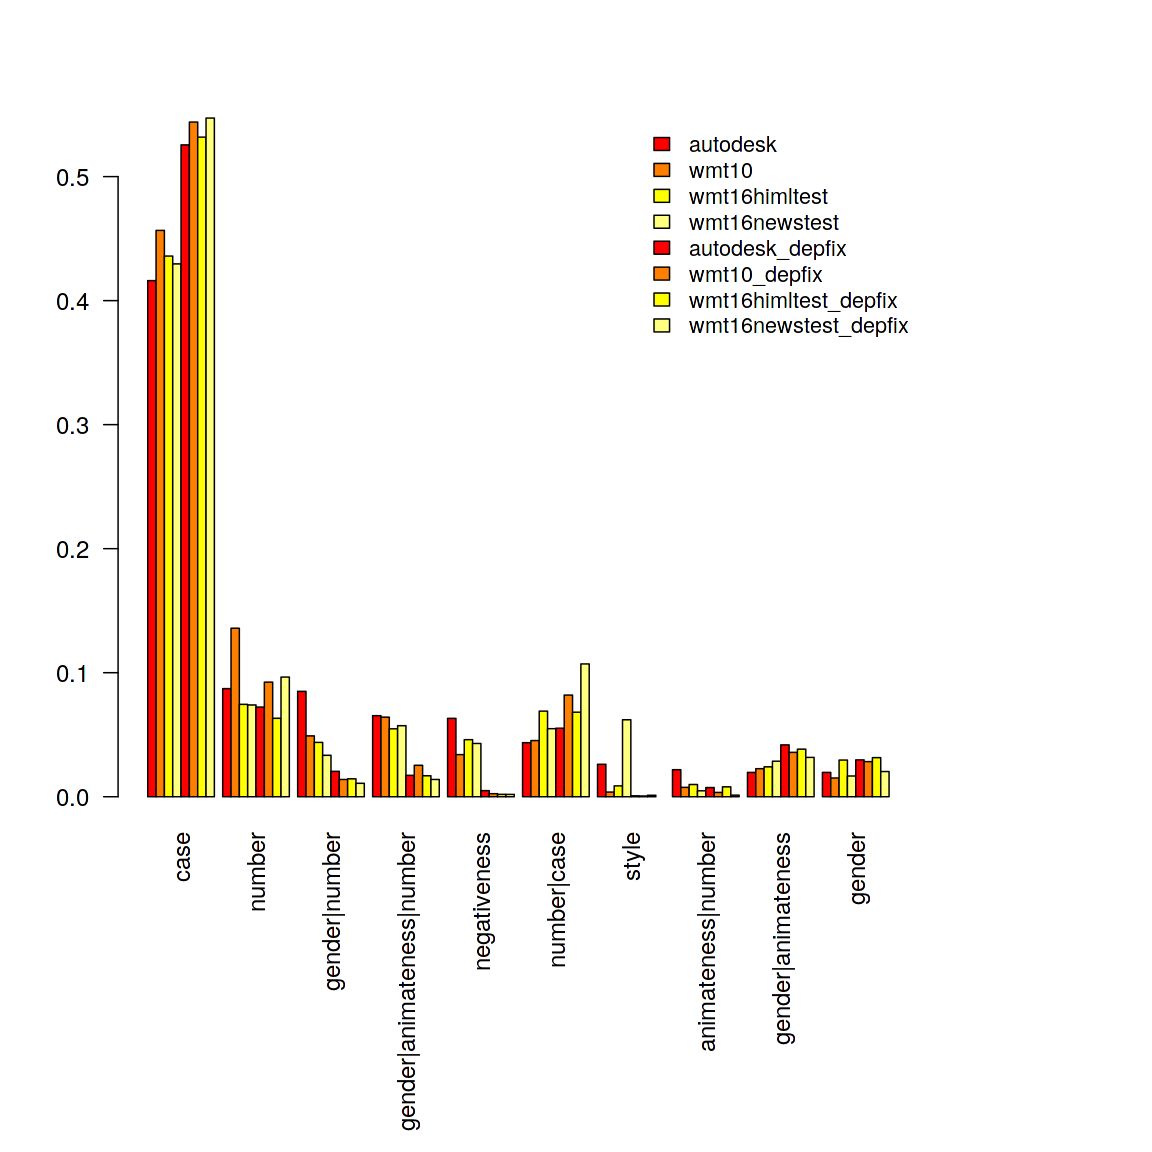
\includegraphics[scale=0.7]{iset}
  \caption{
    Frequency of the most changed Interset categories, grouped by a datasets. Categories containing
    "\textbar" symbol (e.g. gender\textbar{}number) represent changes made simultaneously.
}
  \label{iset-barplot}
\end{figure}

% with source
\begin{figure}
\centering
  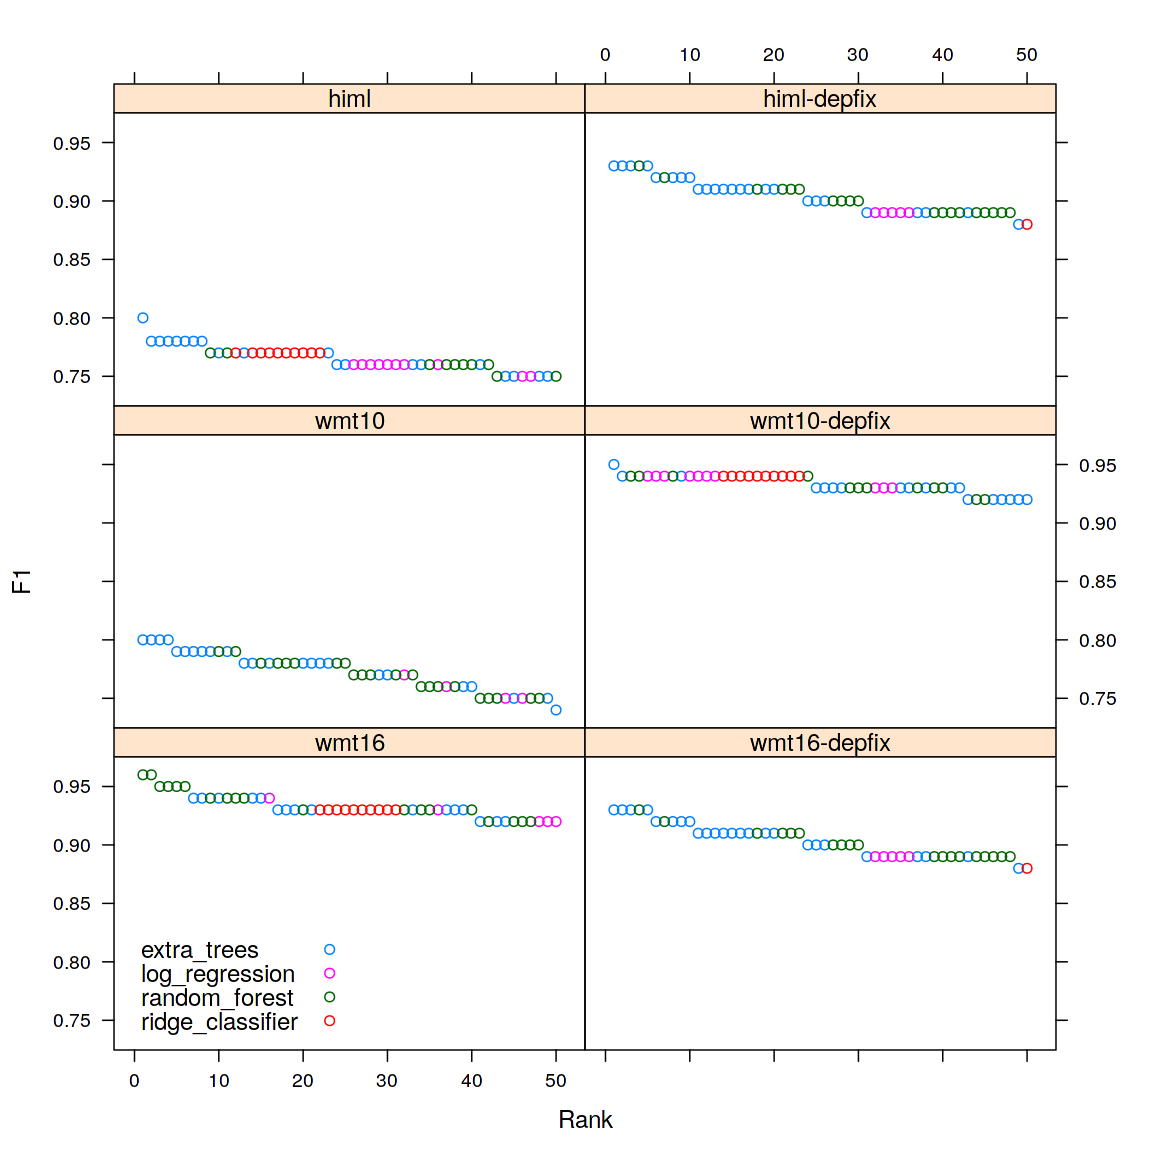
\includegraphics[scale=0.7]{cat-class}
  \caption{
    Overview of the classifier performance (category prediction).
We have tried several variations of the hyperparameters
for each classifier. The classifiers are ordered from the best to the worst. Only top 50 results
are shown for each dataset.
}
  \label{cats-draft}
\end{figure}

\subsection{Feature selection}

We have decided to perform additional feature selection with models trained on the standard HimL dataset
and WMT10 dataset because there is still a reasonable room for an improvement. Again, we have tried two initial features
sets, one using the source side features and one without them. We have not noticed any significant difference in performance
between models trained on these two initial feature sets\footnote{Only difference was that the extremely randomized
trees performed sligly better than the random forest classifier if they both used the smaller feature set.} so we decided to use the larger one and leave
the feature selection to the separate model.

We have compared several methods of feature selection: KBest selection
(with chi-squared scoring function), selection based on lasso regularization and selection through
models (svm, random forest). Again, we have done a rough comparison of these methods, by trying out
several parameter configurations. We tested them on a model with a fixed parameters. The results
are in~\Fref{cats-sel}. We can see that with the HimL dataset, the feature selection did not have
any positive influence on the resulting model. On the other hand, we have decided to use the KBest
feature filtering for the WMT10 dataset model training.

\begin{figure}
\centering
  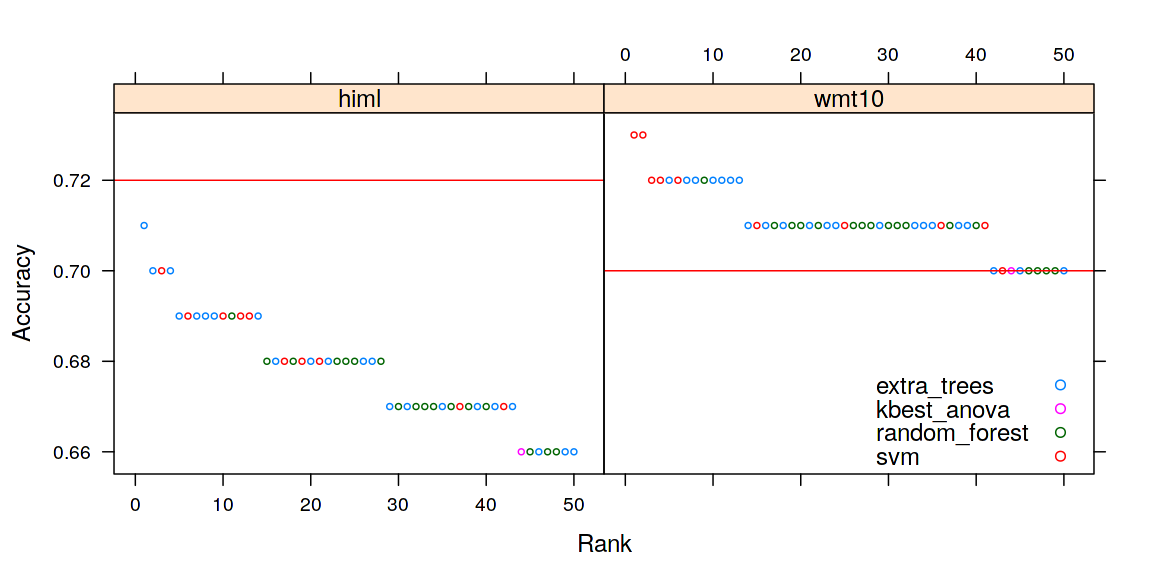
\includegraphics[scale=0.7]{cat-sel}
  \caption{
    Overview of the random forest performance when combined with various feature selection methods.
The methods are ordered from the best to the worst. The horizontal line marks the best performance without
a feature selection method. Only top 50 results are shown for each dataset.
}
  \label{cats-sel}
\end{figure}

%\subsection{Multitask models}
%todo???

\subsection{Model summary}

In the end, we have trained six different models, one for the each dataset presented in the rough comparison.
The summary of their in-domain final performance is in`\Tref{cats-summary}. Aside from the case clasiffier, we have also compared performance
of the chosen multitask classifiers: the case-number (CN) and case-number-gender (CNG) classifier and the case-number-gender-animateness (CNGA)
classifier.
These classifiers were trained using the same ML methods, each one was tuned separately.
%okec - zhorseny perf. s pridavanim cat?

\todo{tohle az do final evaluace?}
Since the domains of the datasets differ to a various degree, we have decided to combine the models trained
on the different datasets, however, we do not combine different types of classifier. This combined model
compares result of each separate classifier (with the prediction probability) and picks the most probable choice.

